%%%%%%%%%%%%%%%%%%%%%%%
% Comp 170, Fall 2019
% Homework 4
% Author: Vladimir Hugec
%%%%%%%%%%%%%%%%%%%%%%%

% This portion of the LaTeX document are configuration 
% You can see it as all the #includes in C++
\documentclass[12pt]{article}

\usepackage{epsfig}
\usepackage{amsmath}
\usepackage{amsthm}
\usepackage{listings}
\usepackage{graphicx}
\usepackage{tikz}

\newtheorem{lemma}{Lemma}
\newtheorem{theorem}{Theorem}

\usepackage{titlesec}
\titleformat{\section}
{\normalfont\Large\bfseries}{Question~\thesection:}{1em}{}

\newlength{\toppush}
\setlength{\toppush}{2\headheight}
\addtolength{\toppush}{\headsep}

\def\subjnum{Comp 170}
\def\subjname{Computation Theory}

\def\doheading#1#2#3{\vfill\eject\vspace*{-\toppush}%
  \vbox{\hbox to\textwidth{{\bf} \subjnum: \subjname \hfil Vladimir Hugec}%
    \hbox to\textwidth{{\bf} Tufts University, Fall 2019 \hfil#3\strut}%
    \hrule}}


\newcommand{\htitle}[1]{\vspace*{1.25ex plus 1ex minus 0ex}%
\begin{center}
{\large\bf #1}
\end{center}} 


%%%%%%%%%%%%%%%%%%%%%%%%%%%%%%%%%%%%%%%%%%%%%%%%%%%%%%%%%%%%%%%%%%%
% BEGIN DOCUMENT
%%%%%%%%%%%%%%%%%%%%%%%%%%%%%%%%%%%%%%%%%%%%%%%%%%%%%%%%%%%%%%%%%%%
\begin{document}
\doheading{2}{title}{Homework 4}

\section{}

$G = \{V, \Sigma, S, P\}$

$V = \{S, A, B\}$

$\Sigma = \{x,y,z,w\}$ 

and P is:

$\indent S\rightarrow AB$

$\indent A \rightarrow xAy$   $|$  $\epsilon$

$\indent B \rightarrow zBw$    $|$  $\epsilon$

$\newline$
My grammar is not ambiguous since for generating any string $w$ of the form $x^m y^m z^n w^n$ there is only one S which can be used.

\pagebreak

\section{}

Derivation Tree 1:

\begin{center}
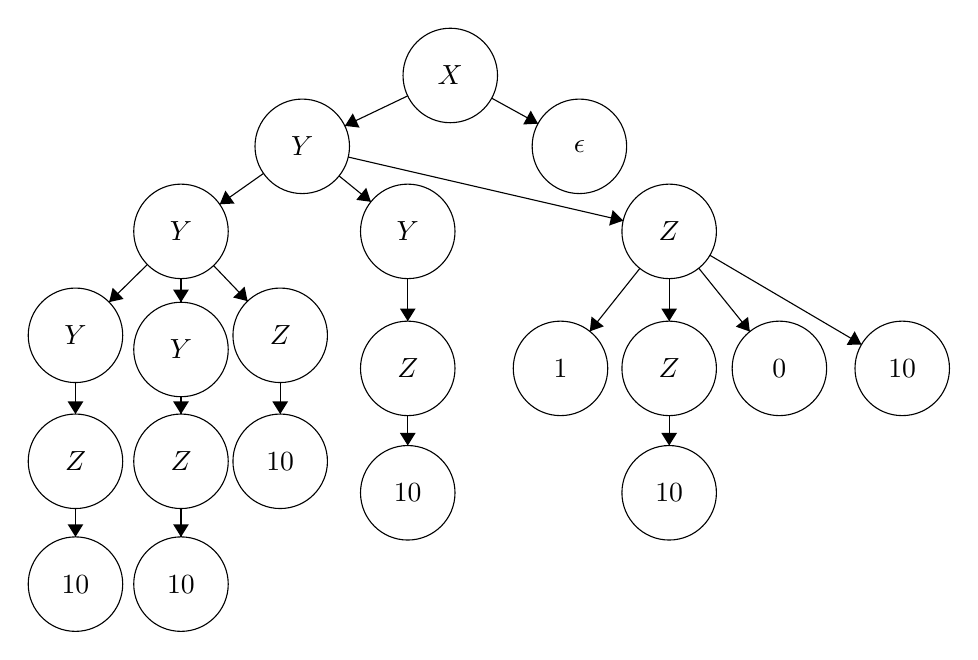
\begin{tikzpicture}[scale=0.2]
\tikzstyle{every node}+=[inner sep=0pt]
\draw [black] (39.3,-4.1) circle (3);
\draw (39.3,-4.1) node {$X$};
\draw [black] (29.9,-8.6) circle (3);
\draw (29.9,-8.6) node {$Y$};
\draw [black] (22.2,-14) circle (3);
\draw (22.2,-14) node {$Y$};
\draw [black] (36.6,-14) circle (3);
\draw (36.6,-14) node {$Y$};
\draw [black] (53.2,-14) circle (3);
\draw (53.2,-14) node {$Z$};
\draw [black] (47.5,-8.6) circle (3);
\draw (47.5,-8.6) node {$\epsilon$};
\draw [black] (46.3,-22.7) circle (3);
\draw (46.3,-22.7) node {$1$};
\draw [black] (53.2,-22.7) circle (3);
\draw (53.2,-22.7) node {$Z$};
\draw [black] (60.2,-22.7) circle (3);
\draw (60.2,-22.7) node {$0$};
\draw [black] (68,-22.7) circle (3);
\draw (68,-22.7) node {$10$};
\draw [black] (53.2,-30.6) circle (3);
\draw (53.2,-30.6) node {$10$};
\draw [black] (36.6,-22.7) circle (3);
\draw (36.6,-22.7) node {$Z$};
\draw [black] (36.6,-30.6) circle (3);
\draw (36.6,-30.6) node {$10$};
\draw [black] (15.5,-20.6) circle (3);
\draw (15.5,-20.6) node {$Y$};
\draw [black] (15.5,-28.6) circle (3);
\draw (15.5,-28.6) node {$Z$};
\draw [black] (22.2,-21.5) circle (3);
\draw (22.2,-21.5) node {$Y$};
\draw [black] (28.5,-20.6) circle (3);
\draw (28.5,-20.6) node {$Z$};
\draw [black] (28.5,-28.6) circle (3);
\draw (28.5,-28.6) node {$10$};
\draw [black] (22.2,-28.6) circle (3);
\draw (22.2,-28.6) node {$Z$};
\draw [black] (22.2,-36.4) circle (3);
\draw (22.2,-36.4) node {$10$};
\draw [black] (15.5,-36.4) circle (3);
\draw (15.5,-36.4) node {$10$};
\draw [black] (36.59,-5.4) -- (32.61,-7.3);
\fill [black] (32.61,-7.3) -- (33.54,-7.41) -- (33.11,-6.51);
\draw [black] (41.93,-5.54) -- (44.87,-7.16);
\fill [black] (44.87,-7.16) -- (44.41,-6.33) -- (43.93,-7.21);
\draw [black] (27.44,-10.32) -- (24.66,-12.28);
\fill [black] (24.66,-12.28) -- (25.6,-12.23) -- (25.02,-11.41);
\draw [black] (32.24,-10.48) -- (34.26,-12.12);
\fill [black] (34.26,-12.12) -- (33.96,-11.23) -- (33.33,-12);
\draw [black] (32.82,-9.28) -- (50.28,-13.32);
\fill [black] (50.28,-13.32) -- (49.61,-12.65) -- (49.39,-13.63);
\draw [black] (53.2,-25.7) -- (53.2,-27.6);
\fill [black] (53.2,-27.6) -- (53.7,-26.8) -- (52.7,-26.8);
\draw [black] (51.34,-16.35) -- (48.16,-20.35);
\fill [black] (48.16,-20.35) -- (49.05,-20.03) -- (48.27,-19.41);
\draw [black] (53.2,-17) -- (53.2,-19.7);
\fill [black] (53.2,-19.7) -- (53.7,-18.9) -- (52.7,-18.9);
\draw [black] (55.08,-16.34) -- (58.32,-20.36);
\fill [black] (58.32,-20.36) -- (58.21,-19.43) -- (57.43,-20.05);
\draw [black] (55.79,-15.52) -- (65.41,-21.18);
\fill [black] (65.41,-21.18) -- (64.98,-20.34) -- (64.47,-21.21);
\draw [black] (36.6,-17) -- (36.6,-19.7);
\fill [black] (36.6,-19.7) -- (37.1,-18.9) -- (36.1,-18.9);
\draw [black] (36.6,-25.7) -- (36.6,-27.6);
\fill [black] (36.6,-27.6) -- (37.1,-26.8) -- (36.1,-26.8);
\draw [black] (20.06,-16.11) -- (17.64,-18.49);
\fill [black] (17.64,-18.49) -- (18.56,-18.29) -- (17.86,-17.58);
\draw [black] (15.5,-23.6) -- (15.5,-25.6);
\fill [black] (15.5,-25.6) -- (16,-24.8) -- (15,-24.8);
\draw [black] (22.2,-17) -- (22.2,-18.5);
\fill [black] (22.2,-18.5) -- (22.7,-17.7) -- (21.7,-17.7);
\draw [black] (24.27,-16.17) -- (26.43,-18.43);
\fill [black] (26.43,-18.43) -- (26.24,-17.51) -- (25.51,-18.2);
\draw [black] (28.5,-23.6) -- (28.5,-25.6);
\fill [black] (28.5,-25.6) -- (29,-24.8) -- (28,-24.8);
\draw [black] (22.2,-24.5) -- (22.2,-25.6);
\fill [black] (22.2,-25.6) -- (22.7,-24.8) -- (21.7,-24.8);
\draw [black] (22.2,-31.6) -- (22.2,-33.4);
\fill [black] (22.2,-33.4) -- (22.7,-32.6) -- (21.7,-32.6);
\draw [black] (15.5,-31.6) -- (15.5,-33.4);
\fill [black] (15.5,-33.4) -- (16,-32.6) -- (15,-32.6);
\end{tikzpicture}
\end{center}

Derivation Tree 2:

\begin{center}
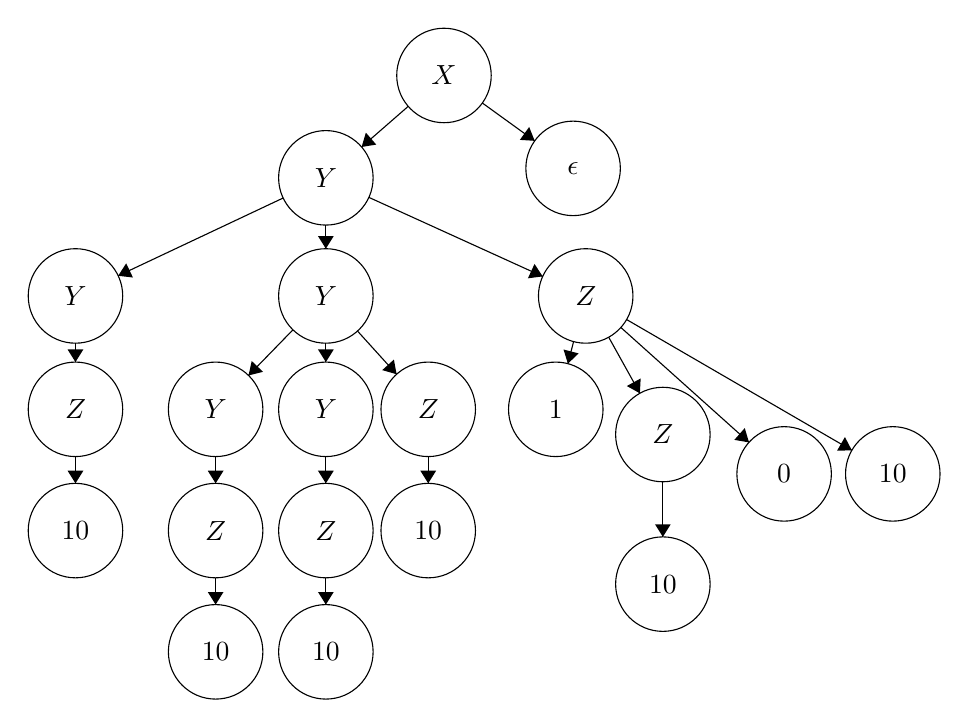
\begin{tikzpicture}[scale=0.2]
\tikzstyle{every node}+=[inner sep=0pt]
\draw [black] (39.3,-4.1) circle (3);
\draw (39.3,-4.1) node {$X$};
\draw [black] (31.8,-10.6) circle (3);
\draw (31.8,-10.6) node {$Y$};
\draw [black] (31.8,-18.1) circle (3);
\draw (31.8,-18.1) node {$Y$};
\draw [black] (15.9,-18.1) circle (3);
\draw (15.9,-18.1) node {$Y$};
\draw [black] (48.3,-18.1) circle (3);
\draw (48.3,-18.1) node {$Z$};
\draw [black] (47.5,-10) circle (3);
\draw (47.5,-10) node {$\epsilon$};
\draw [black] (46.4,-25.3) circle (3);
\draw (46.4,-25.3) node {$1$};
\draw [black] (53.2,-26.9) circle (3);
\draw (53.2,-26.9) node {$Z$};
\draw [black] (60.9,-29.4) circle (3);
\draw (60.9,-29.4) node {$0$};
\draw [black] (67.8,-29.4) circle (3);
\draw (67.8,-29.4) node {$10$};
\draw [black] (53.2,-36.4) circle (3);
\draw (53.2,-36.4) node {$10$};
\draw [black] (15.9,-25.3) circle (3);
\draw (15.9,-25.3) node {$Z$};
\draw [black] (15.9,-33) circle (3);
\draw (15.9,-33) node {$10$};
\draw [black] (24.8,-25.3) circle (3);
\draw (24.8,-25.3) node {$Y$};
\draw [black] (24.8,-33) circle (3);
\draw (24.8,-33) node {$Z$};
\draw [black] (31.8,-25.3) circle (3);
\draw (31.8,-25.3) node {$Y$};
\draw [black] (38.3,-25.3) circle (3);
\draw (38.3,-25.3) node {$Z$};
\draw [black] (38.3,-33) circle (3);
\draw (38.3,-33) node {$10$};
\draw [black] (31.8,-33) circle (3);
\draw (31.8,-33) node {$Z$};
\draw [black] (31.8,-40.7) circle (3);
\draw (31.8,-40.7) node {$10$};
\draw [black] (24.8,-40.7) circle (3);
\draw (24.8,-40.7) node {$10$};
\draw [black] (37.03,-6.06) -- (34.07,-8.64);
\fill [black] (34.07,-8.64) -- (35,-8.49) -- (34.34,-7.73);
\draw [black] (41.74,-5.85) -- (45.06,-8.25);
\fill [black] (45.06,-8.25) -- (44.71,-7.37) -- (44.12,-8.19);
\draw [black] (31.8,-13.6) -- (31.8,-15.1);
\fill [black] (31.8,-15.1) -- (32.3,-14.3) -- (31.3,-14.3);
\draw [black] (29.09,-11.88) -- (18.61,-16.82);
\fill [black] (18.61,-16.82) -- (19.55,-16.93) -- (19.12,-16.03);
\draw [black] (34.53,-11.84) -- (45.57,-16.86);
\fill [black] (45.57,-16.86) -- (45.05,-16.07) -- (44.63,-16.98);
\draw [black] (53.2,-29.9) -- (53.2,-33.4);
\fill [black] (53.2,-33.4) -- (53.7,-32.6) -- (52.7,-32.6);
\draw [black] (47.53,-21) -- (47.17,-22.4);
\fill [black] (47.17,-22.4) -- (47.85,-21.75) -- (46.89,-21.5);
\draw [black] (49.76,-20.72) -- (51.74,-24.28);
\fill [black] (51.74,-24.28) -- (51.79,-23.34) -- (50.91,-23.82);
\draw [black] (50.53,-20.1) -- (58.67,-27.4);
\fill [black] (58.67,-27.4) -- (58.4,-26.49) -- (57.74,-27.24);
\draw [black] (50.9,-19.6) -- (65.2,-27.9);
\fill [black] (65.2,-27.9) -- (64.76,-27.06) -- (64.26,-27.93);
\draw [black] (15.9,-21.1) -- (15.9,-22.3);
\fill [black] (15.9,-22.3) -- (16.4,-21.5) -- (15.4,-21.5);
\draw [black] (15.9,-28.3) -- (15.9,-30);
\fill [black] (15.9,-30) -- (16.4,-29.2) -- (15.4,-29.2);
\draw [black] (29.71,-20.25) -- (26.89,-23.15);
\fill [black] (26.89,-23.15) -- (27.81,-22.92) -- (27.09,-22.23);
\draw [black] (24.8,-28.3) -- (24.8,-30);
\fill [black] (24.8,-30) -- (25.3,-29.2) -- (24.3,-29.2);
\draw [black] (31.8,-21.1) -- (31.8,-22.3);
\fill [black] (31.8,-22.3) -- (32.3,-21.5) -- (31.3,-21.5);
\draw [black] (33.81,-20.33) -- (36.29,-23.07);
\fill [black] (36.29,-23.07) -- (36.12,-22.14) -- (35.38,-22.81);
\draw [black] (38.3,-28.3) -- (38.3,-30);
\fill [black] (38.3,-30) -- (38.8,-29.2) -- (37.8,-29.2);
\draw [black] (31.8,-28.3) -- (31.8,-30);
\fill [black] (31.8,-30) -- (32.3,-29.2) -- (31.3,-29.2);
\draw [black] (31.8,-36) -- (31.8,-37.7);
\fill [black] (31.8,-37.7) -- (32.3,-36.9) -- (31.3,-36.9);
\draw [black] (24.8,-36) -- (24.8,-37.7);
\fill [black] (24.8,-37.7) -- (25.3,-36.9) -- (24.3,-36.9);
\end{tikzpicture}
\end{center}

\textbf{A)} 

By Definition 2.7 in the TextBook, the grammar that uses rule set $R_{1}$ is ambiguous. It generates a string $w$ ambiguously since it has two different leftmost derivations making the grammar ambiguous as shown above in Derivation Tree \#1 and \#2.

$\newline$

\textbf{B)}
To show that $R_{2}$ is not ambiguous, we can take a look at the grammar's constituent parts.

$X \rightarrow Y | \epsilon$, this cannot be ambiguous, since using the left most variable always yeilds $Y$ so there is no choice and therefore not ambiguous.

$Y \rightarrow ZY | Z$, there is also no ambiguity here since at a time only one can be used, unlike in $R_{1}$ where there are two $Y$'s leading to choices and ambiguity, so here there are no choices and therefore again no ambiguity.

$Z \rightarrow 1Z0 | 10$, here, again for the same reasons as above, there is no ambiguity.

\pagebreak

\section{}

\begin{center}
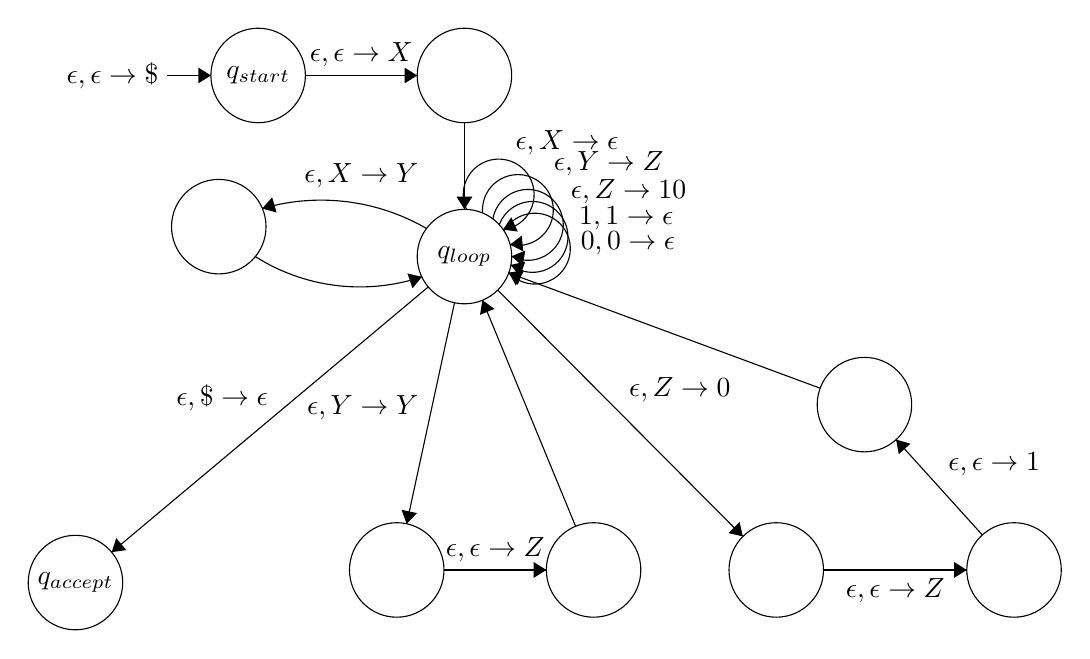
\begin{tikzpicture}[scale=0.2]
\tikzstyle{every node}+=[inner sep=0pt]
\draw [black] (18.3,-9.8) circle (3);
\draw (18.3,-9.8) node {$q_{start}$};
\draw [black] (31.4,-9.8) circle (3);
\draw [black] (31.4,-21.3) circle (3);
\draw (31.4,-21.3) node {$q_{loop}$};
\draw [black] (15.8,-19.4) circle (3);
\draw [black] (27.1,-41.2) circle (3);
\draw [black] (39.6,-41.2) circle (3);
\draw [black] (51.2,-41.2) circle (3);
\draw [black] (66.3,-41.2) circle (3);
\draw [black] (56.8,-30.7) circle (3);
\draw [black] (6.7,-42) circle (3);
\draw (6.7,-42) node {$q_{accept}$};
\draw [black] (12.5,-9.8) -- (15.3,-9.8);
\draw (12,-9.8) node [left] {$\epsilon,\epsilon \rightarrow \$$};
\fill [black] (15.3,-9.8) -- (14.5,-9.3) -- (14.5,-10.3);
\draw [black] (21.3,-9.8) -- (28.4,-9.8);
\fill [black] (28.4,-9.8) -- (27.6,-9.3) -- (27.6,-10.3);
\draw (24.85,-9.3) node [above] {$\epsilon,\epsilon \rightarrow X$};
\draw [black] (31.4,-12.8) -- (31.4,-18.3);
\fill [black] (31.4,-18.3) -- (31.9,-17.5) -- (30.9,-17.5);
\draw [black] (18.563,-18.247) arc (106.21371:59.89803:13.361);
\fill [black] (18.56,-18.25) -- (19.47,-18.5) -- (19.19,-17.54);
\draw (24.85,-17) node [above] {$\epsilon,X \rightarrow Y$};
\draw [black] (28.698,-22.586) arc (-71.48757:-122.4007:12.401);
\fill [black] (28.7,-22.59) -- (27.78,-22.37) -- (28.1,-23.31);
\draw [black] (31.537,-18.315) arc (205.10153:-82.89847:2.25);
\draw (37.91,-14.88) node [above] {$\epsilon,X \rightarrow \epsilon$};
\fill [black] (33.85,-19.59) -- (34.79,-19.71) -- (34.37,-18.8);
\draw [black] (30.77,-24.23) -- (27.73,-38.27);
\fill [black] (27.73,-38.27) -- (28.39,-37.59) -- (27.41,-37.38);
\draw (28.5,-30.89) node [left] {$\epsilon,Y \rightarrow Y$};
\draw [black] (30.1,-41.2) -- (36.6,-41.2);
\fill [black] (36.6,-41.2) -- (35.8,-40.7) -- (35.8,-41.7);
\draw (33.35,-40.7) node [above] {$\epsilon,\epsilon \rightarrow Z$};
\draw [black] (32.553,-18.543) arc (185.04238:-102.95762:2.25);
\draw (37.04,-15.42) node [right] {$\epsilon,Y \rightarrow Z$};
\fill [black] (34.29,-20.54) -- (35.13,-20.97) -- (35.04,-19.97);
\draw [black] (38.46,-38.43) -- (32.54,-24.07);
\fill [black] (32.54,-24.07) -- (32.39,-25) -- (33.31,-24.62);
\draw [black] (33.52,-23.43) -- (49.08,-39.07);
\fill [black] (49.08,-39.07) -- (48.87,-38.15) -- (48.17,-38.86);
\draw (41.82,-29.77) node [right] {$\epsilon,Z \rightarrow 0$};
\draw [black] (54.2,-41.2) -- (63.3,-41.2);
\fill [black] (63.3,-41.2) -- (62.5,-40.7) -- (62.5,-41.7);
\draw (58.75,-41.7) node [below] {$\epsilon,\epsilon \rightarrow Z$};
\draw [black] (64.29,-38.98) -- (58.81,-32.92);
\fill [black] (58.81,-32.92) -- (58.98,-33.85) -- (59.72,-33.18);
\draw (62.09,-34.49) node [right] {$\epsilon,\epsilon \rightarrow 1$};
\draw [black] (53.99,-29.66) -- (34.21,-22.34);
\fill [black] (34.21,-22.34) -- (34.79,-23.09) -- (35.14,-22.15);
\draw [black] (33.205,-18.919) arc (170.56505:-117.43495:2.25);
\draw (38.13,-17.17) node [right] {$\epsilon,Z \rightarrow 10$};
\fill [black] (34.39,-21.28) -- (35.1,-21.91) -- (35.26,-20.92);
\draw [black] (29.1,-23.23) -- (9,-40.07);
\fill [black] (9,-40.07) -- (9.93,-39.94) -- (9.29,-39.18);
\draw (16.01,-31.16) node [above] {$\epsilon,\$ \rightarrow \epsilon$};
\draw [black] (33.608,-19.286) arc (160.10437:-127.89563:2.25);
\draw (38.65,-18.86) node [right] {$1,1 \rightarrow \epsilon$};
\fill [black] (34.34,-21.83) -- (34.92,-22.57) -- (35.26,-21.63);
\draw [black] (33.915,-19.686) arc (150.43165:-137.56835:2.25);
\draw (38.76,-20.43) node [right] {$0,0 \rightarrow \epsilon$};
\fill [black] (34.21,-22.31) -- (34.66,-23.14) -- (35.15,-22.27);
\end{tikzpicture}
\end{center}


\end{document}
%%%%%%%%%%%%%%%%%%%%%%%%%%%%%%%%%%%%%%%%%%%%%%%%%%%%%%%%%%%%%%%%%%%%%%

